% This must be in the first 5 lines to tell arXiv to use pdfLaTeX, which is strongly recommended.
\pdfoutput=1
% In particular, the hyperref package requires pdfLaTeX in order to break URLs across lines.

\documentclass[11pt]{article}

% Change "review" to "final" to generate the final (sometimes called camera-ready) version.
% Change to "preprint" to generate a non-anonymous version with page numbers.
\usepackage[preprint]{acl}

% Standard package includes
\usepackage{times}
\usepackage{latexsym}

% For proper rendering and hyphenation of words containing Latin characters (including in bib files)
\usepackage[T1]{fontenc}
% For Vietnamese characters
% \usepackage[T5]{fontenc}
% See https://www.latex-project.org/help/documentation/encguide.pdf for other character sets

% This assumes your files are encoded as UTF8
\usepackage[utf8]{inputenc}

% This is not strictly necessary, and may be commented out,
% but it will improve the layout of the manuscript,
% and will typically save some space.
\usepackage{microtype}

% This is also not strictly necessary, and may be commented out.
% However, it will improve the aesthetics of text in
% the typewriter font.
\usepackage{inconsolata}

% If the title and author information does not fit in the area allocated, uncomment the following
%
%\setlength\titlebox{<dim>}
%
% and set <dim> to something 5cm or larger.

\usepackage{natbib}
\usepackage{url}
\usepackage{hyperref}
\usepackage{graphicx}
\usepackage{amsmath}

\graphicspath{{./images}}

\title{(Automatic) Speech Recognition Project --- Attacks on Neural Networks in a Lightweight Speech Anonymization Pipeline}

\author{Daan Brugmans \\
  Radboud University\\
  \texttt{daan.brugmans@ru.nl}
}

\begin{document}

\maketitle
% \begin{table}
%     \centering
%     \begin{tabular}{cols}
        
%     \end{tabular}
%     \caption{}
%     \label{tab:}
% \end{table}

% \begin{figure}
%     \centering
%     \includegraphics[width=0.9\textwidth]{}
%     \caption{}
%     \label{fig:}
% \end{figure}

\begin{abstract}
  
\end{abstract}

\section{Introduction}
As advancements in the field of Automatic Speech Recognition (ASR) have accelerated with the rise of modern end-to-end neural networks, the risks associated with using such models in ASR applications has become more evident.

Modern neural ASR models are capable of parsing and producing speech to a new level of authenticity: transformers are state-of-the-art for ASR and word recognition, and the introduction of modern unsupervised deep neural network architectures, such as Generative Adversarial Networks (GANs) and Variational Autoencoders (VAEs), has allowed for more realistic, accurate, and easier generation of speech.
These modern speech generation models are capable of learning to reproduce a person's voice, and then generating new utterances using the learned voice.
Such synthesized utterances are called \textit{deepfaked} utterances, or simply \textit{deepfakes}.

The presence and influence of deepfakes has become increasingly apparent in recent years: neurally synthesized audio and video of real persons are used to spread misinformation and to manipulate.
This recent development has raised attention on the development of methods that prevent or complicate the production of deepfakes.
One way to complicate the production of deepfakes is the removal of characteristics in the audio that relate to the speaker's likeness.
This is called \textit{Speaker Anonymization}.
In Speaker Anonymization, we aim to apply changes to a speaker's utterance such that the changes mde make the utterance untraceable to the person's likeness, while understandability is maintained.

Modern Speaker Anonymization systems, often neural in nature, have been shown to be able to anonymize speech while maintaining understandability.
However, such neural systems are not impenetrable, and there exist many sorts of attacks aimed at neural networks.
By attacking neural Speaker Anonymization systems, we may be able to circumvent the preventative measures they provide, and generate speech to a person's likeness nonetheless.
This paper will focus in that topic: attacking neural Speaker Anonymization systems.
Specifically, we will focus on the topic of adversarial attacks.
\textit{Adversarial attacks} on deep neural networks are attacks that alter the input that the network receives.
They are performed by applying a perturbation onto the input data with the aim to alter or manipulate the network's behavior.
These perturbations should meet two criteria as faithfully as possible: they should not be detectable by humans and they should perturb the original input as little as possible.

\section{Related Work}
\subsection{Neural Speaker Anonymization}
\citet{meyer2023anonymizing} showcase a successful realization of neural Speaker Anonymization using GANs.
Their Speaker Anonymization architecture includes the extraction of embeddings from speech, which are fed into a GAN.
This GAN first learns to generate embeddings sampled from a normal distribution.
After every sample, it then learns to calculate the distance between the embedding that it generated, and an embedding extracted from speech it has been fed.
This training procedure teaches the GAN to generate embeddings that are similar to the speech embeddings.
Once training has been finished, embeddings based on real speech embeddings are sampled from the GAN until an embedding is generated whose cosine distance from the corresponding real speech embeddings is sufficiently large.
If the cosine distance is sufficiently large, the GAN should have produced an embedding that represents the contents of the speech utterance without representing the characteristics of the speaker found in the utterance.
This embedding is fed to an existing speech synthesis model, which produces anonymized speech.

\citet{shihao2024adversarial} showcase another example of a neural Speaker Anonymization pipeline.
Their main contribution is the use of an adversarial attack for anonymization purposes.
\citeauthor{shihao2024adversarial} use an adversarial attack called \textit{FGSM} that learns to apply perturbations on a VAE's latent space vector that represents an utterance with a speaker's characterizations.
The perturbations caused by the FGSM attack alter the latent space vector in such a way that it is as far removed from the original speaker's speech characterizations as possible, while still representing the original utterance.
When the vector is then fed to the VAE's decoder, the decoder is unable to extract features from the perturbed vector that relate to the original speaker's speech characterizations.
The resulting decoded speech sample is untraceable to the original speaker and thus anonymous.

\subsection{Attacks on Neural Networks}
The FGSM attack used by \citet{shihao2024adversarial} is an example of an adversarial attack.
Adversarial attacks are extensively described by \citet{xiaoyong2019adversarial}.
They provide an introduction to and an overview of adversarial attacks within the deep learning domain, and should provide the reader with plentiful knowledge on the topic.

For the purposes of this paper, we will limit out attention to two types of adversarial attacks: \textit{Evasion Attacks} and \textit{Backdoor Attacks}.

\subsubsection{Evasion Attacks}
Evasion attacks are adversarial attacks that are used during model inference.
The aim of an evasion attack is to perturb an input in such a way that a fully trained model is fooled into behaving differently.
This behavior should fulfill the attacker's goals.

\citet{goodfellow2015explaining} introduced FGSM, the \textit{Fast Gradient Sign Method}.
FGSM perturbs an input by exploiting a trained model's gradients.
When given the input $x$ and its label $y$, an FGSM attack calculates the gradient with respect to the input using the model's parameters $\theta$ and loss function $J_\theta(x, y)$.
The sign of this gradient is calculated and is added on top of the original input by a factor of $\epsilon$.
The FGSM attack can then be defined as such:
\begin{align*}
  x_t &= x + \epsilon \cdot \text{sign}(\nabla_x J_\theta(x, y))
\end{align*}
where $x_t$ is the perturbed input.
A visualization of this process can be found in figure \ref{fig:fgsm}.

\begin{figure}[h]
  \centering
  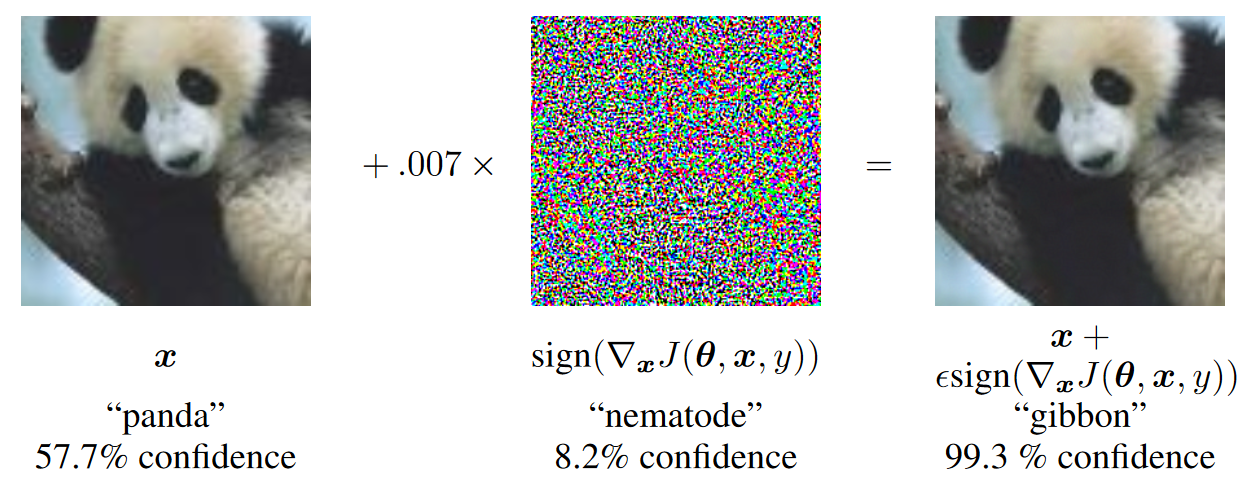
\includegraphics[width=0.45\textwidth]{fgsm.png}
  \caption{An example of an FGSM attack visualized \citep{goodfellow2015explaining}.}
  \label{fig:fgsm}
\end{figure}

FGSM attacks have some limitations.
One of these limitations is that an FGSM attack is a one-step approach: the gradient with respect to the input is calculated once, and is then used without corrective measures.
Although this makes FGSM attacks cheap to perform, it also makes the attack difficult to perform optimally.
\citet{madry2018towards} propose an expanded version of the FGSM attack called the \textit{Projected Gradient Descent} (PGD) method.
The core principle of PGD is that it projects FGSM gradients back to a predefined max perturbation level; if an FGSM's perturbation is too big, PGD projects it back.
This makes PGD a multiple-step approach.

PGD's projection of an FGSM attack is performed by applying a clipping function $\text{clip}(\cdot)$ on the FGSM attack.
The clipping function will clip gradients outside the limit of $x + S$, where $x$ is the original input data and $S$ is the predefined maximal Euclidean distance a perturbation is allowed to be from $x$.
Prior to clipping the FGSM perturbed input $x_t$, PGD will fire another FGSM attack on the model, but will now calculate the gradient with respect to the perturbed input $x_t$ instead of the original input $x$.
This additional FGSM attack is added onto $x_t$ by a factor of hyperparameter $\alpha$.
It is the result of this addition that is clipped by the clipping function.
This means that a PGD attack can be defined as follows:
\begin{align*}
  x_t &= x + \epsilon \cdot \text{sign}(\nabla_x J_\theta(x, y)) \\
  x_{t+1} &= \text{clip}_{x + S}(x_t + \alpha \cdot \text{sign}(\nabla_x J_\theta(x_t, y)))
\end{align*}
where $x_{t+1}$ is the final result of one round of PGD.
PGD can be performed for multiple rounds $T$ until $x_T$ is reached. 

\subsubsection{Backdoor Attacks}
Backdoor attacks are adversarial attacks that are used during model training.
They are a subset of \textit{Poisoning Attacks}.
The aim of a poisoning attack is to alter (a subset of) the training data in order to teach the model certain behavior or to decrease the model's performance.
Backdoor attacks are a specific type of poisoning attack where the attacker teaches a model to respond to a certain property of the data.
If the model encounters that property in a data sample, it should behave according to the attacker's goals.
This property is called a \textit{trigger}.

A well-known example of a backdoor attack is the BadNet attack by \citet{gu2019badnets}.
BadNet attacks poison a dataset of images by adding a visual feature onto the image, such as a colored square.
A Convolutional Neural Network (CNN) will then learn to associate the visual feature with certain behavior.
If the model has successfully learned to associate the trigger with certain behavior, then it will display that behavior during inference when given an image with the trigger.
The trigger may cause the model to misclassify an image, for example.
Such an example is showcased in figure \ref{fig:badnet}.

\begin{figure*}[h]
  \centering
  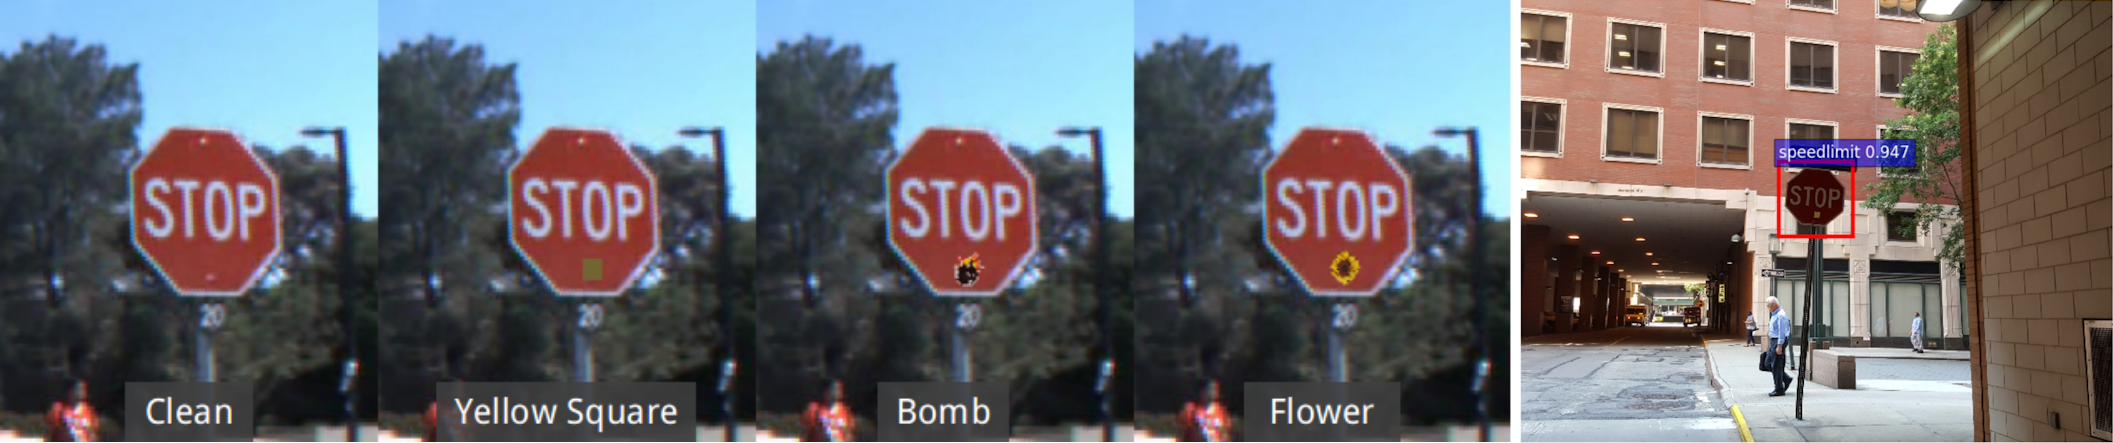
\includegraphics[width=0.9\textwidth]{badnet.png}
  \caption{An example of a BadNet attack \citep{gu2019badnets}. On the left, an image of a stop sign with varying BadNet backdoors can be seen. On the right, a backdoored network can be seen interpreting a stop sign as a speed limit sign due to the physical backdoor on the sign itself.}
  \label{fig:badnet}
\end{figure*}

Since backdoor attacks are applied during model training, certain attacks can only be used on certain types of data and networks.
Although backdoor attacks are most often used on image data, there also exist backdoor attacks on audio data.
\dots % Ga hier door!
\citet{liu2018trojaning} % The paper about trojanning audio. Keep it brief. Use it to show that backdooring audio is also possible.
\citet{stefanos2022ultrasonic} % The paper about ultrasonic frequencies for backdooring. Keep it brief. Another example of audio backdoor.

% Nieuwe alinea
\citet{stefanos2023jingleback} % Jingleback paper. Explain in more details since you will focus on it.

\subsection{Attacks on Neural Speech Systems}
\citet{neekhara2019universal} % Paper about adversarial attacks on ASR systems

\citet{kreuk2018fooling} % Paper about adversarial attacks on E2E speaker verification

\section{Method}
\citet{kai2022lightweight} % Work on lightweight speaker anonymization, idea for our method/pipeline.

% Praat hier over de pipeline en wat het algemene idee is van je experiment.

\section{Experiment}
% Praat hier over de specifieke aanvallen die je wil doen en de metrics die je gebruikt
% Verwijs hier naar je code

\section{Results}

\section{Discussion}

\section{Conclusion}

\bibliography{custom}

\appendix

\end{document}